\chapter{Results and Discussion}
\label{ch:results}

In this chapter, we present the results of the trend detection experiment
described in Chapter \ref{ch:data}. we show the quality of the trend detection
algorithm using ROC curves and distributions of detection time relative to the
true trend onset. we analyze the effect of the algorithm parameters on the
tradeoff between false positive rate, true positive rate, and relative detection
time. Finally, we propose parameter regimes appropriate for three situations: 1)
the cost of a false positive outweighs the cost of a false negative, 2) the cost
of a false negative outweighs the cost of a false positive, and 3) the costs of
a false positive and a false negative are comparable.

\section{Summary of Results}

In this section we show the ROC curve envelopes for each parameter of our
detection algorithm, as well as histograms of relative trend detection time
compared to the true onset of trends, and discuss tradeoffs between true postive
rate, false positive rate, and relative detection time. We demonstrate that in
many cases we are able to detect trends earlier than Twitter while maintaining a
low rate of error.

\subsection{ROC Curve Envelopes}
By varying a single parameter and keeping the rest fixed, we generate a Receiver
Operating Characteristics (ROC) curve that describes the tradeoff between False
Positive Rate (FPR) and True Positive Rate (TPR). Figures \ref{fig:roc_env1} and
\ref{fig:roc_env2} show the ROC curves that result from varying each detection
parameter, aggregated over all combinations of the remaining parameters. The
left side of each plot shows all ROC curves for a given variable parameter
overlayed on a single set of axes. The right side shows the upper-right-most
envelope of those ROC curves, representing the best-case, or achievable ROC
curve.

%TODO: Uncomment
%\begin{comment}
\begin{figure}[!h]
\begin{center}
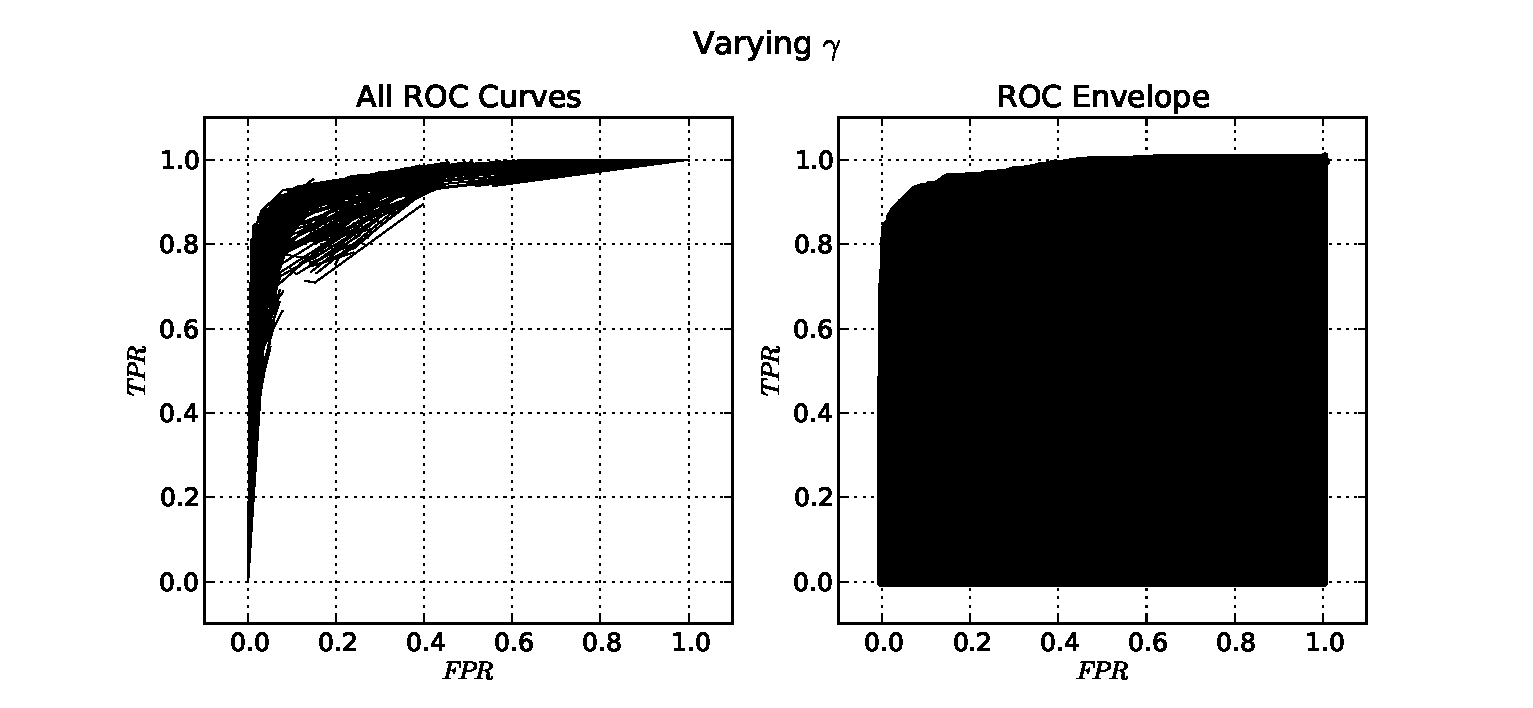
\includegraphics[height=2.5in]{../fig/final/roc_env/gamma}
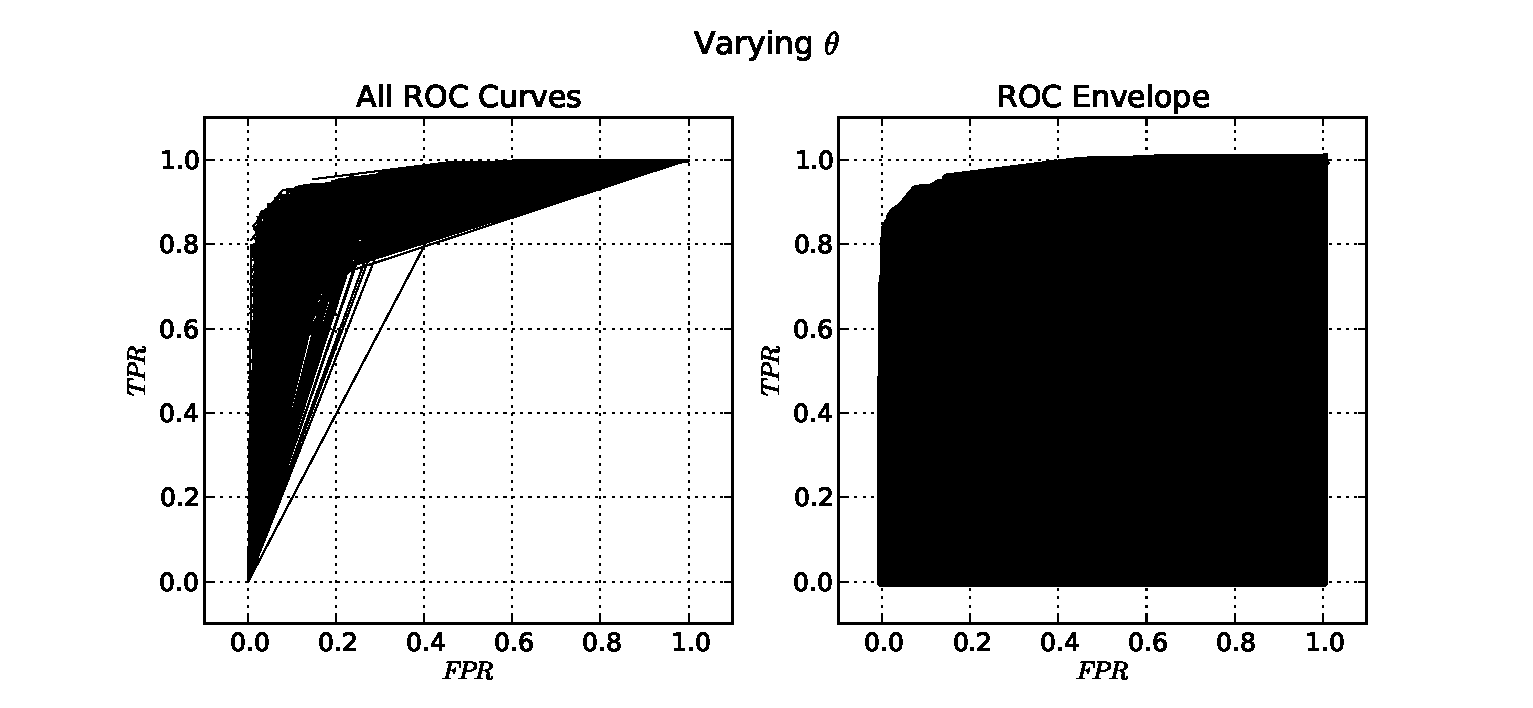
\includegraphics[height=2.5in]{../fig/final/roc_env/theta}
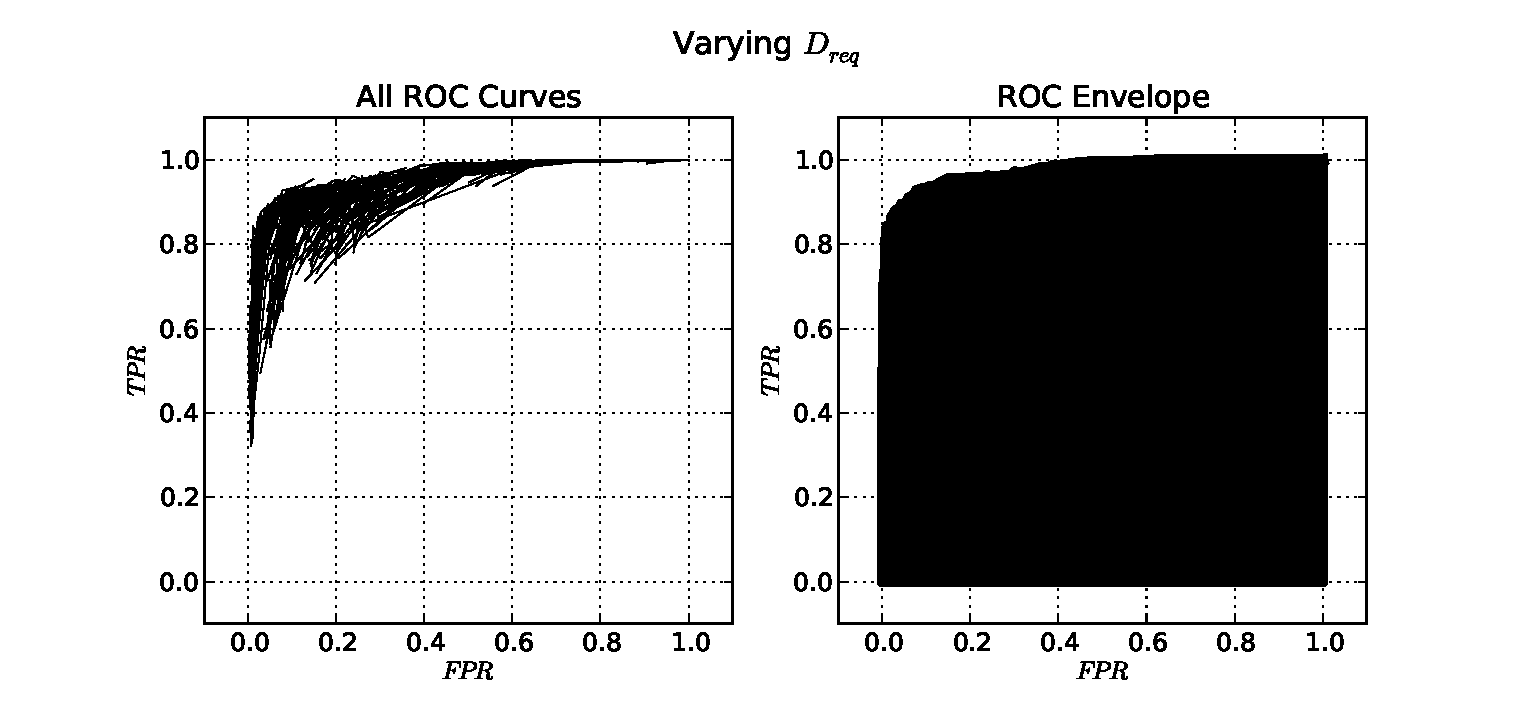
\includegraphics[height=2.5in]{../fig/final/roc_env/dreq}
\end{center}
\caption{\label{fig:roc_env2} {\bf Left}: All ROC curves for the given variable
  parameter overlayed on a single set of axes. {\bf Right}: The upper-right-most
  envelope of those ROC curves, representing the best-case, or achievable ROC
  curve.  }
\end{figure}

\begin{figure}[!h]
\begin{center}
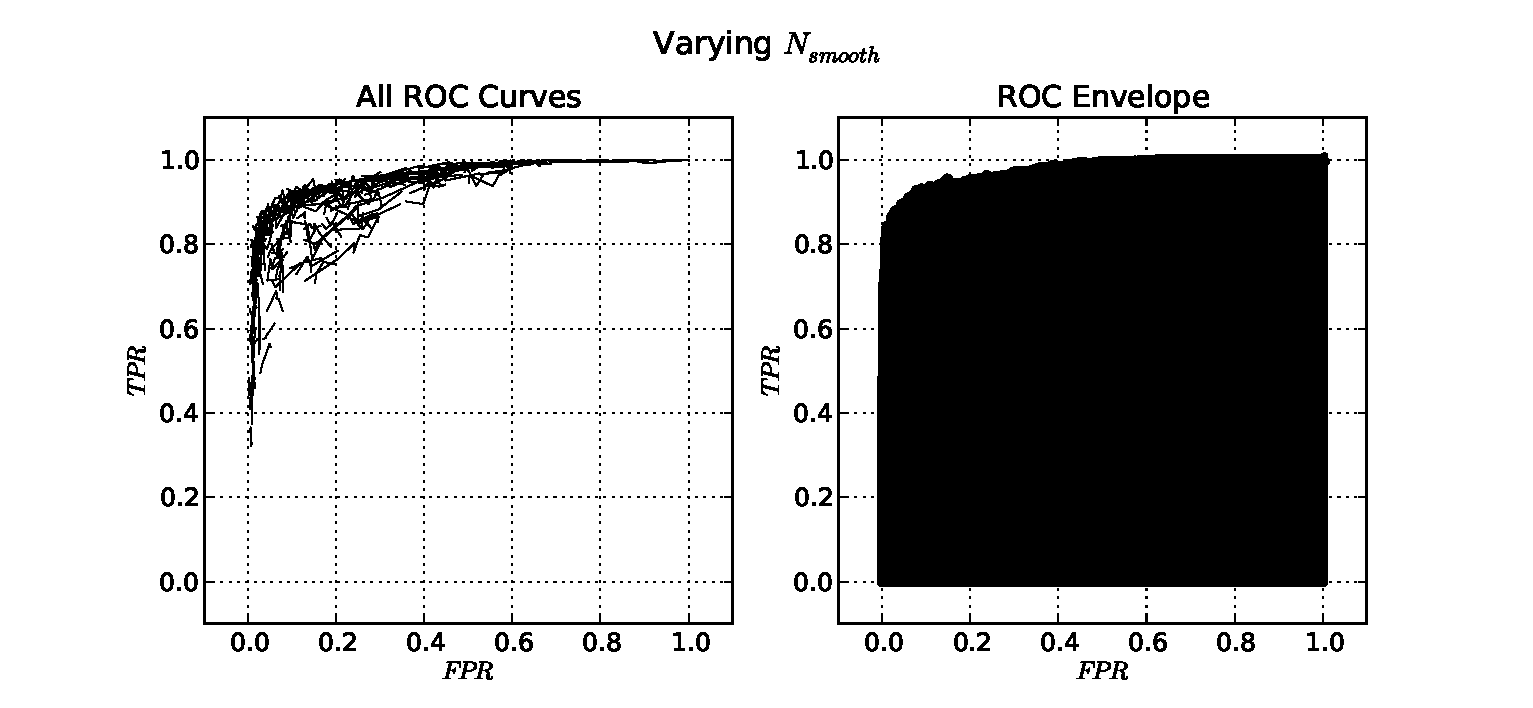
\includegraphics[height=2.5in]{../fig/final/roc_env/Nsmooth}
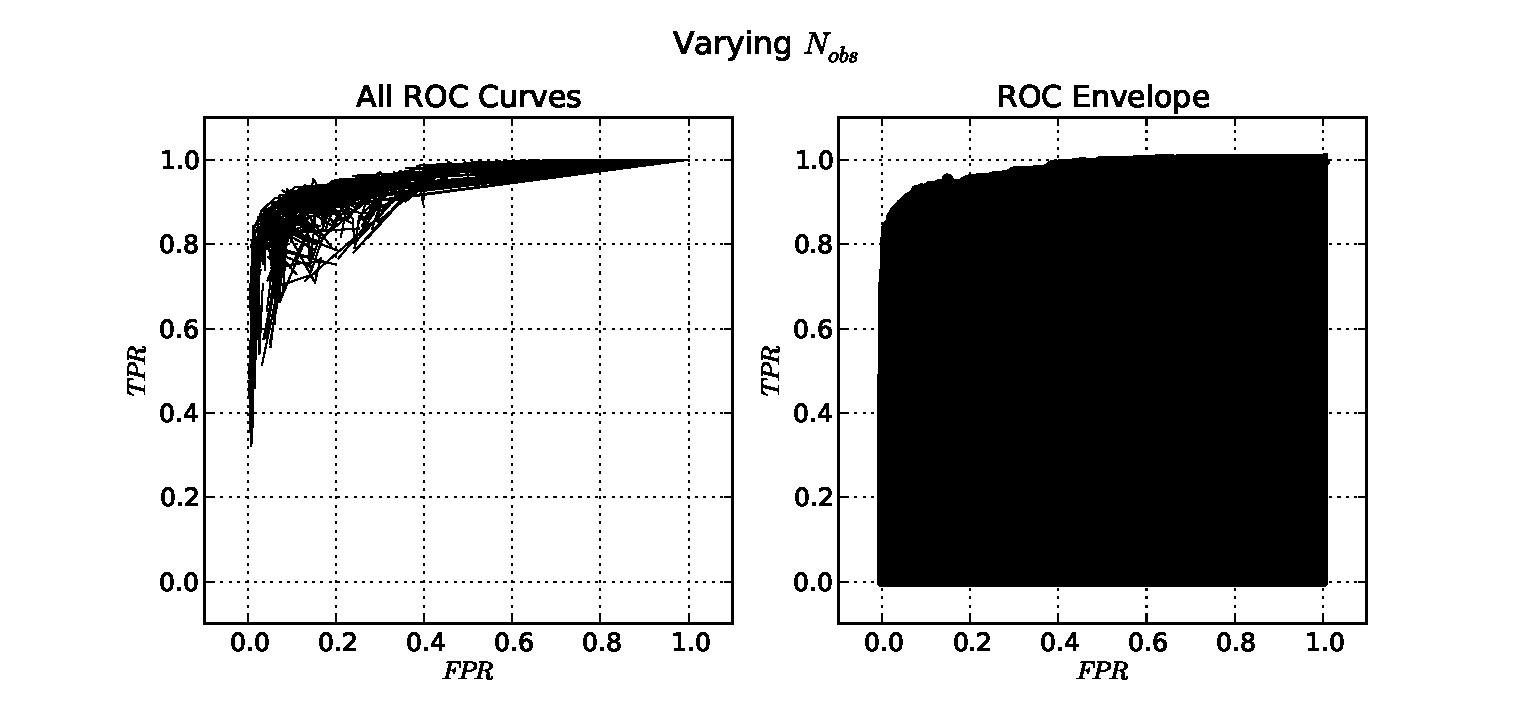
\includegraphics[height=2.5in]{../fig/final/roc_env/nobs}
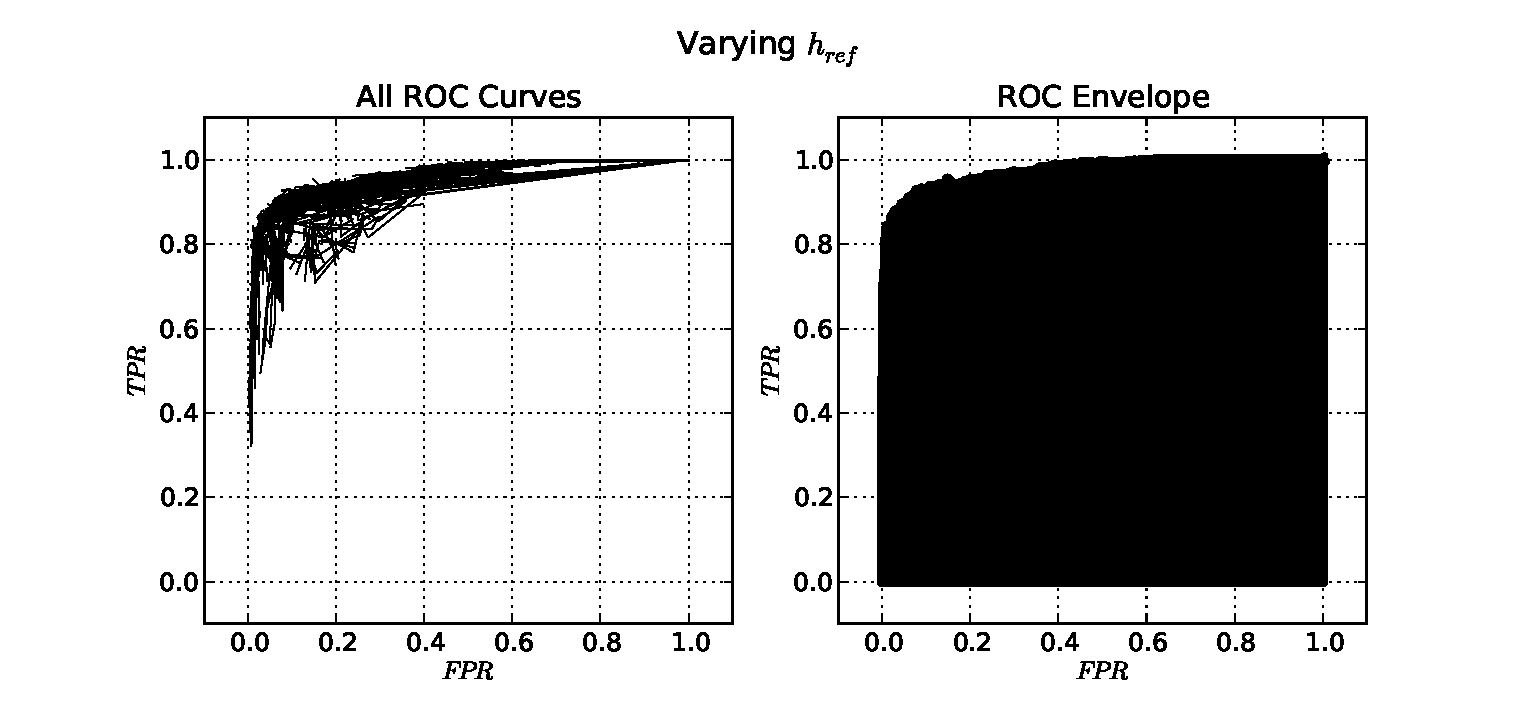
\includegraphics[height=2.5in]{../fig/final/roc_env/href}
\end{center}
\caption{\label{fig:roc_env1}  {\bf Left}: All ROC curves for the given variable
  parameter overlayed on a single set of axes. {\bf Right}: The upper-right-most
  envelope of those ROC curves, representing the best-case, or achievable ROC
  curve.  }
\end{figure}
%\end{comment}

\clearpage
\subsection{Relative Detection Time}
Figure \ref{fig:early_vs_roc} shows the effect of position along the ROC curve
on the relative detection times of our algorithm compared to Twitter's trend
detection algorithm. To simplify our analysis, we break the ROC curve into three
regions: the {\em top} region, referring to the upper right corner of the curve,
the {\em center} region, referring to the upper left corner of the curve, and
the {\em bottom} region, referring to the bottom left corner of the curve. More
precisely, we define the regions as follows.

\begin{defn}[Top region]
$(FPR,TPR)$ is in the top region if $FPR > 0.25$ and $TPR > 0.75$.
\end{defn}
\begin{defn}[Center region]
$(FPR,TPR)$ is in the top region if $FPR \leq 0.25$ and $TPR > 0.75$.
\end{defn}
\begin{defn}[Bottom region]
$(FPR,TPR)$ is in the top region if $FPR \leq 0.25$ and $TPR \leq 0.75$.
\end{defn}

In the top region, we accept the possibility of frequent false detections for
the sake of rarely missing the chance to make a true detection. In the bottom
region, we accept a lower chance of making a true detection for the sake of
rarely making false detections. The center region lies in between these two
extremes. Consequently, points in the top region correspond to earlier detection
relative to the true onset of a trend as detected by Twitter, points in the
bottom, correspond to predominantly late detection, and points in the center
roughly balance being early and late. Figure \ref{fig:early_vs_roc} illustrates this.
\begin{figure}[!h]
\begin{center}
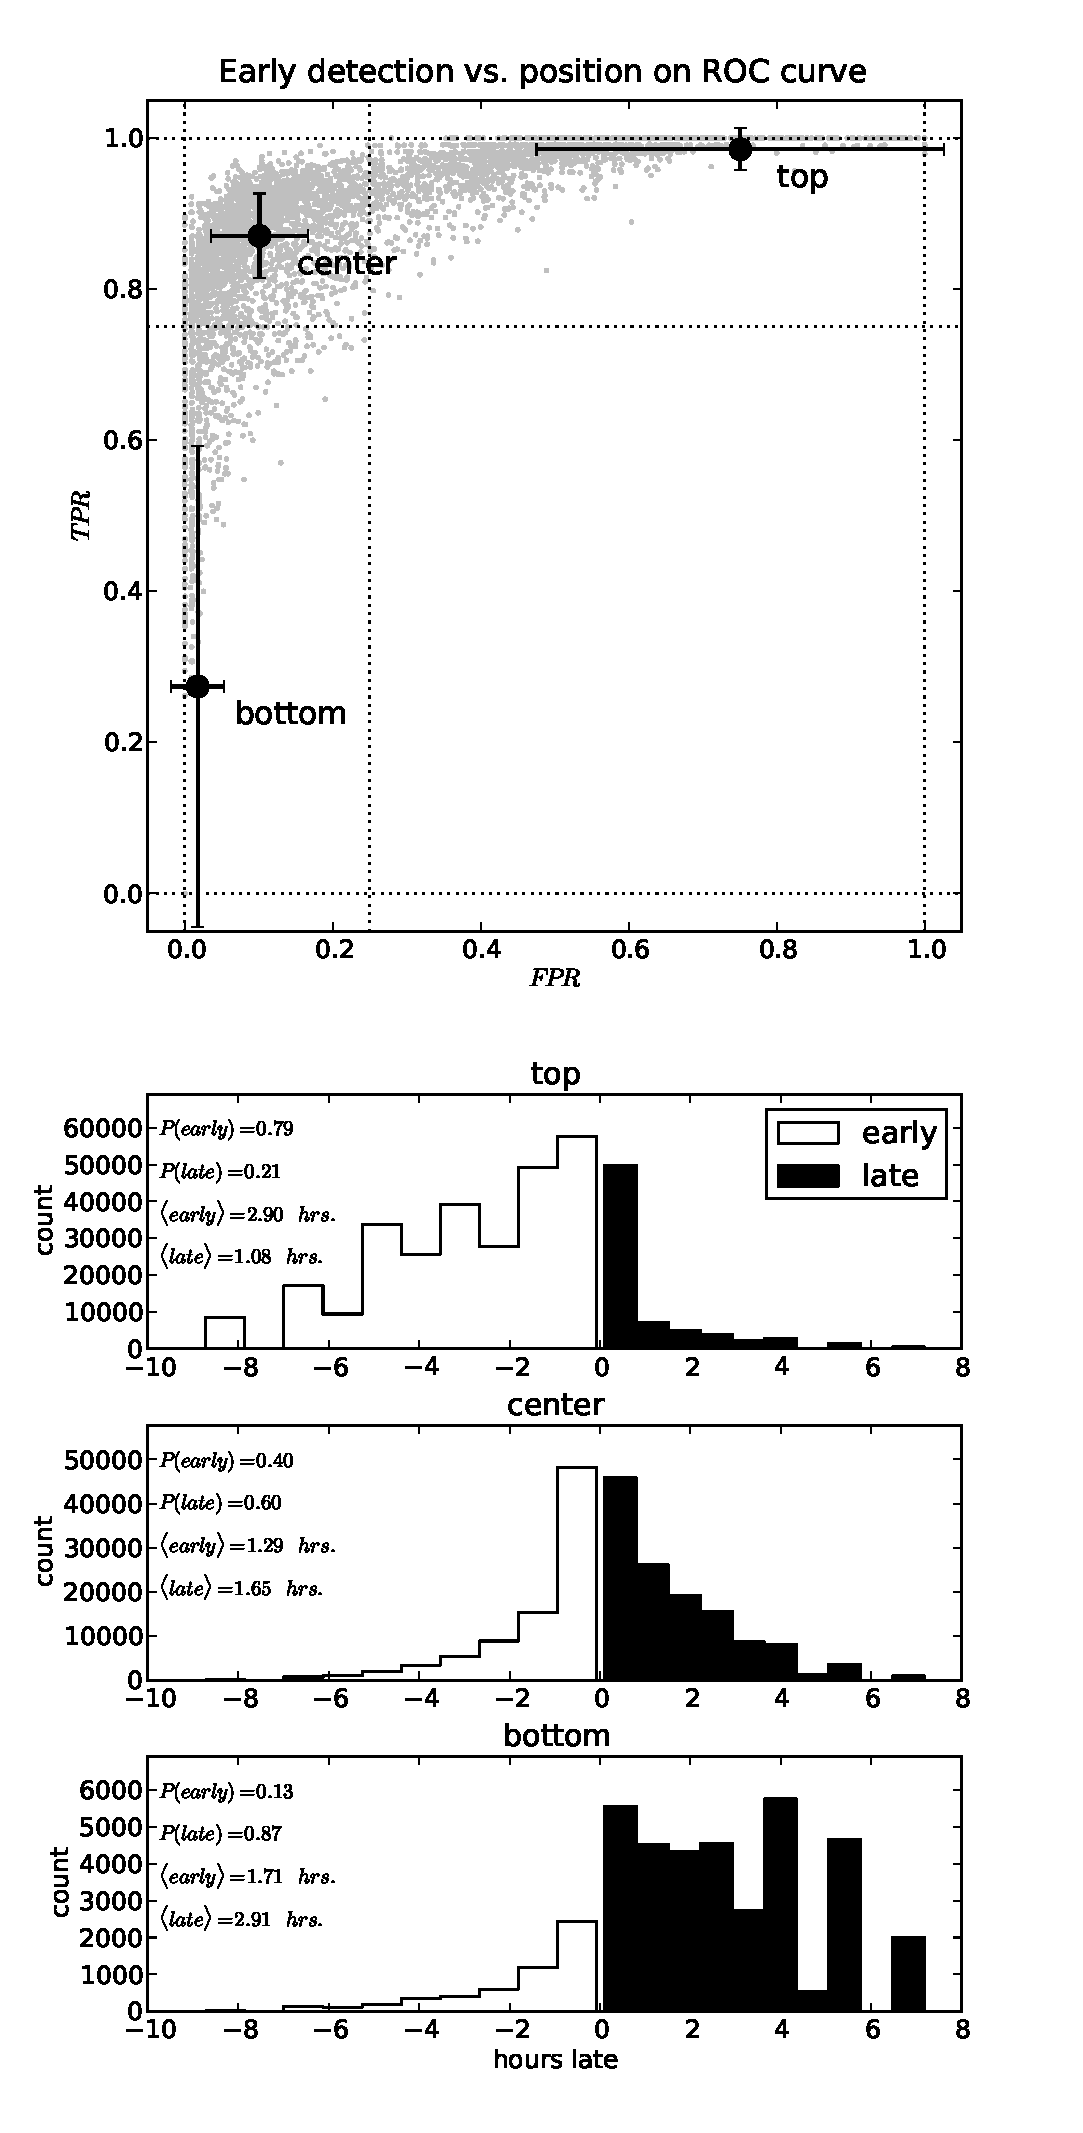
\includegraphics[height=8in]{../fig/final/early_vs_roc}
\end{center}
\caption{\label{fig:early_vs_roc} Effect of position along ROC curve on early
  and late detection.}
\end{figure}

\clearpage
\subsection{Examples} %TODO: Call this something better
In this section, we show examples of our detection algorithm in action on
specific topics. Figure \ref{fig:examples1} shows the detection of fast-spreading
and a slow-spreading topics. In general, it is harder to detect fast-spreading
topics early.

\begin{figure}[!h]
\begin{center}
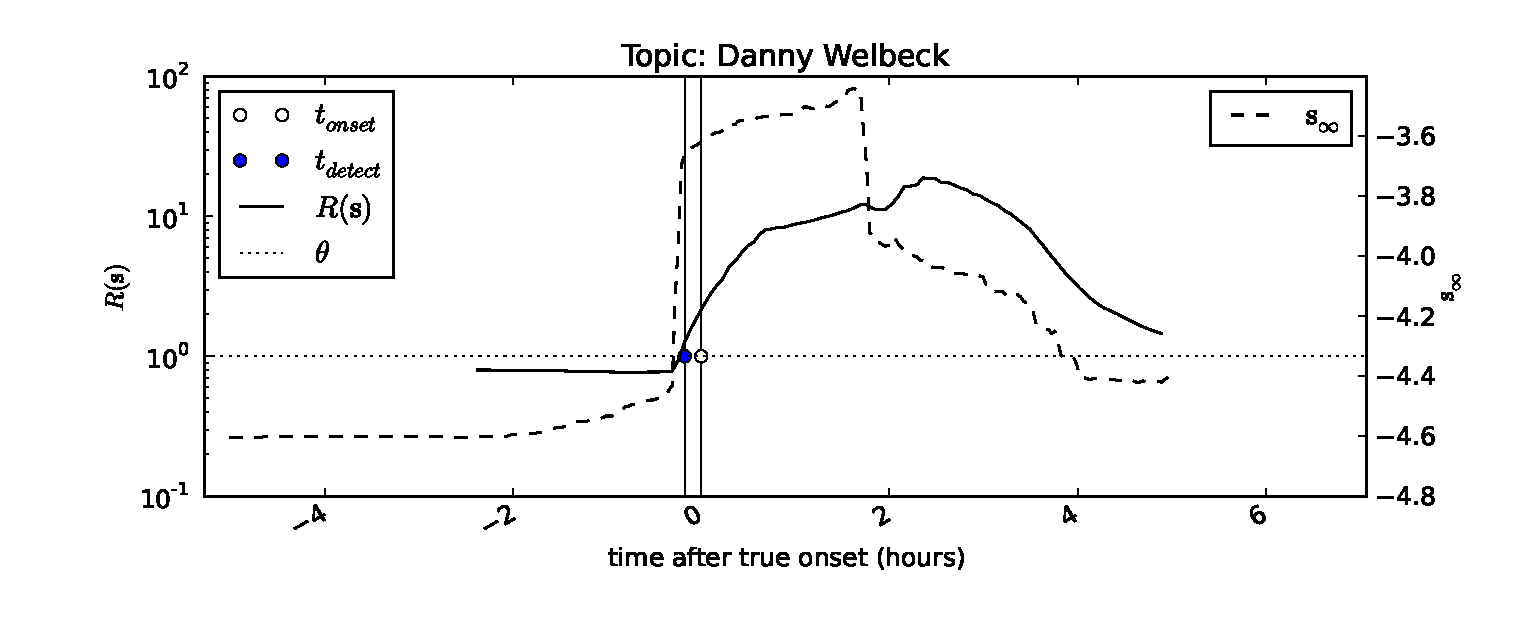
\includegraphics[height=2.5in]{../fig/final/detection_examples/danny_welbeck.eps}
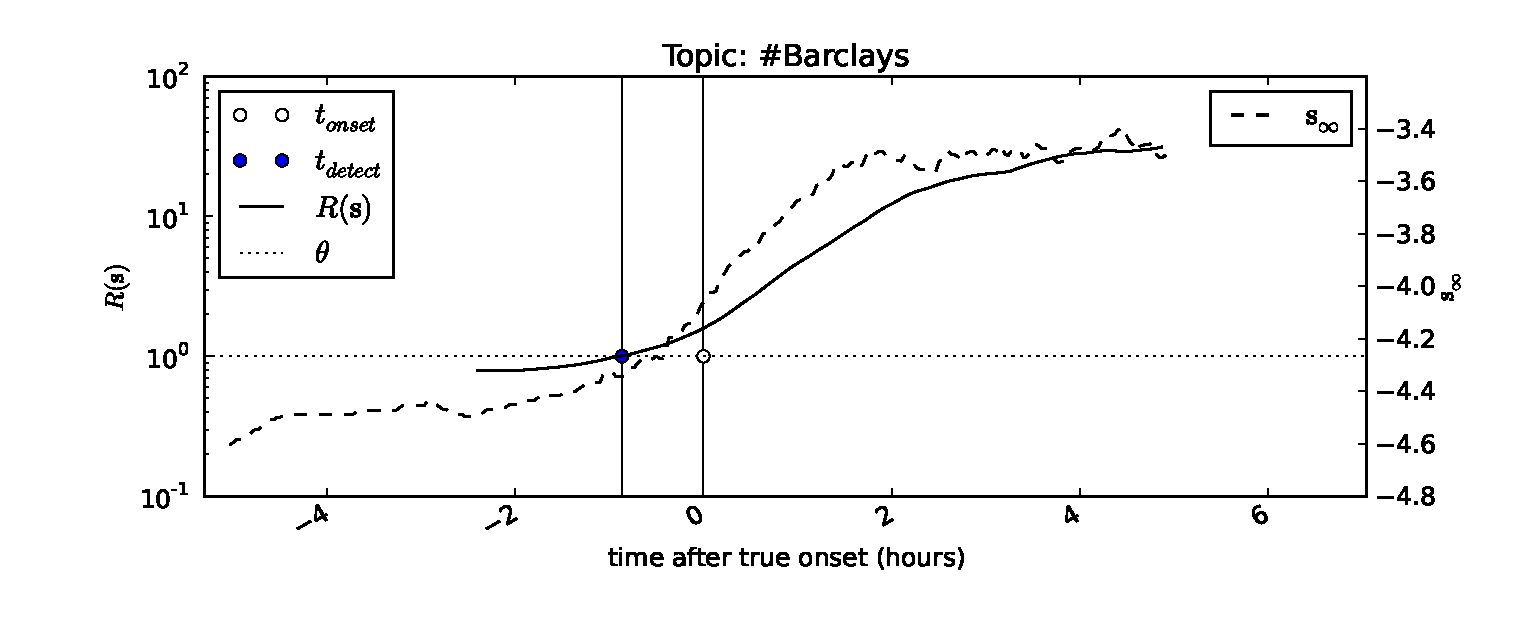
\includegraphics[height=2.5in]{../fig/final/detection_examples/barclays.eps}
\end{center}
\caption{\label{fig:examples1} Fast-spreading vs. slow-spreading topics. {\bf
    Top}: English football player Danny Welbeck scores late in the second half
  of the June 15th match between England and Sweden in the Euro 2012, securing a
  3-2 victory for England. The reaction on Twitter is immediate. {\bf Bottom:}
  Ed Miliband, leader of the UK's Labour Party, calls for a criminal
  investigation of Barclays, the global financial services provider, over
  involvement in the Libor fraud scandal. The story stimulates steadily growing
  discussion over the course of the day.}
\end{figure}

Figure \ref{fig:examples2} shows two true negative topics --- topics that did
not trend and were not detected as trending. In one case, the topic
(``Ludacris'') is a celebrity who, despite receiving consistently high attention
on Twitter, is not involved in any rapidly breaking story, and hence never
becomes a trending topic in the time period considered. The other topic,
``tweetin,'' is presumed to be a common expression that is not associted with
any trending topic.
\begin{figure}[!h]
\begin{center}
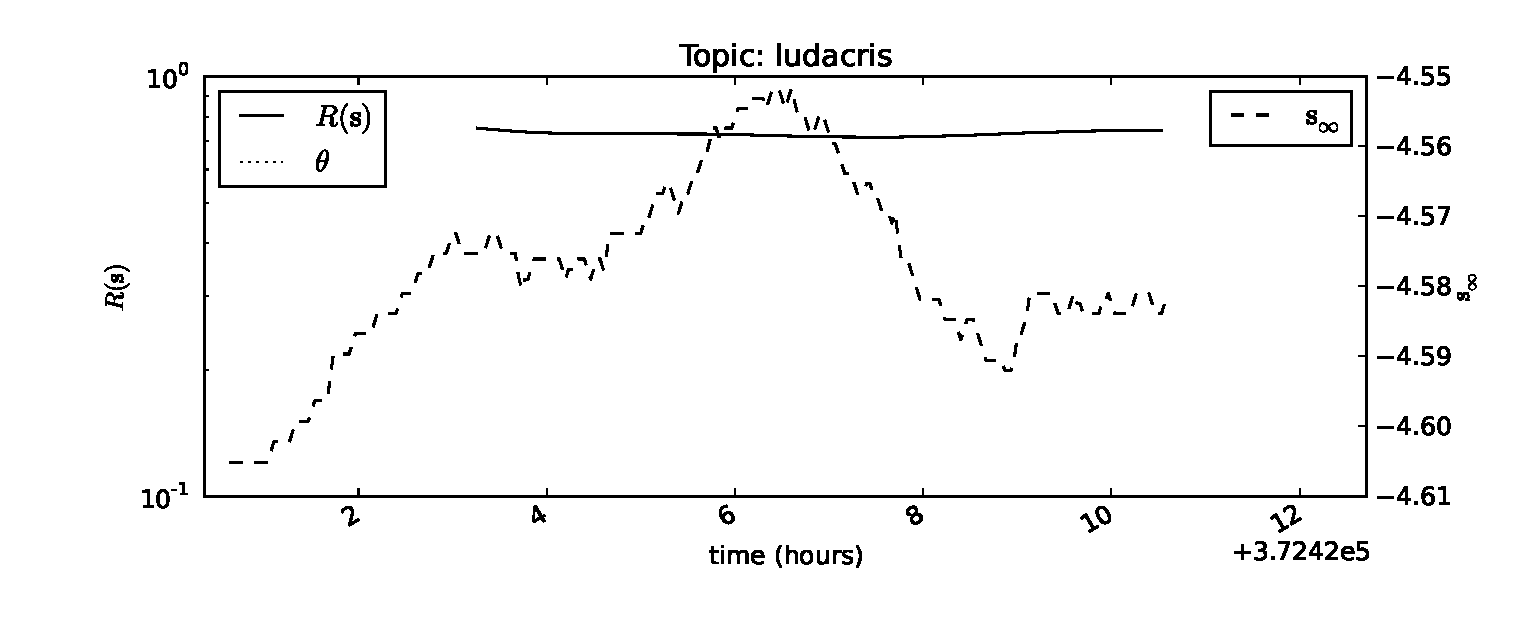
\includegraphics[height=2.5in]{../fig/final/detection_examples/tn/ludacris.eps}
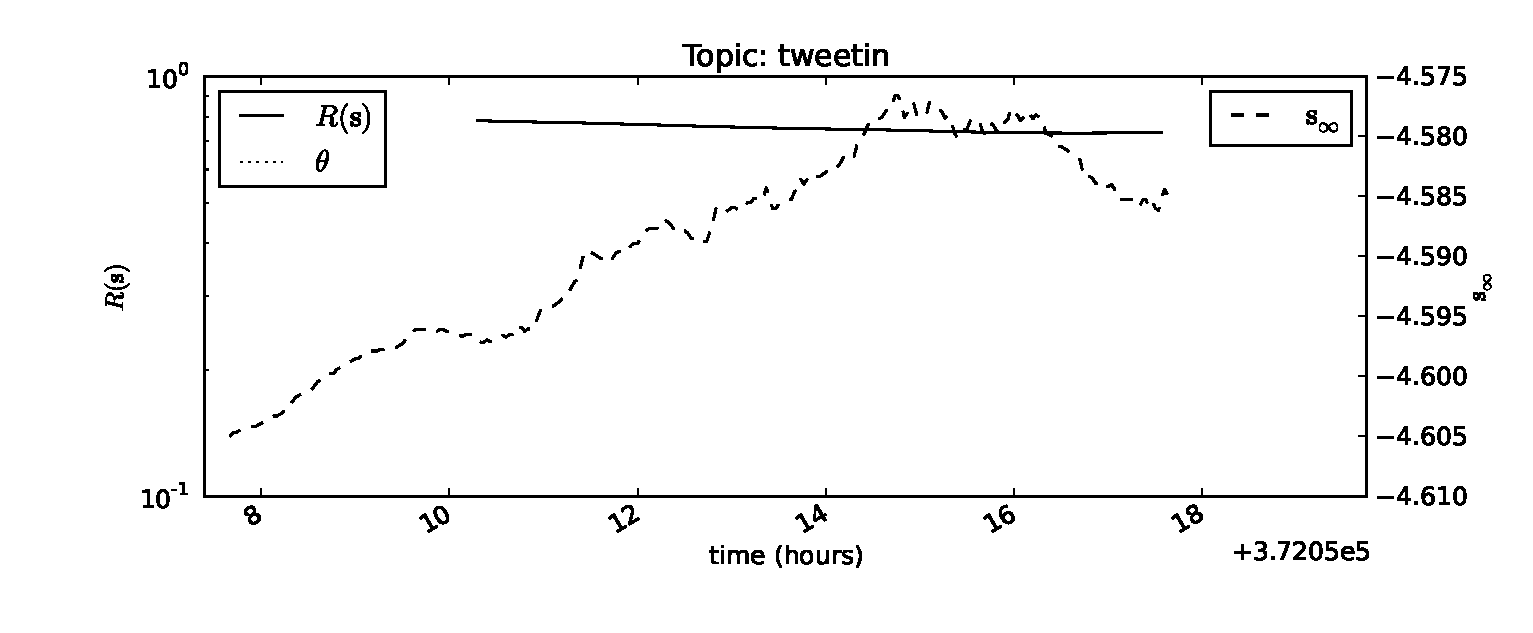
\includegraphics[height=2.5in]{../fig/final/detection_examples/tn/tweetin.eps}
%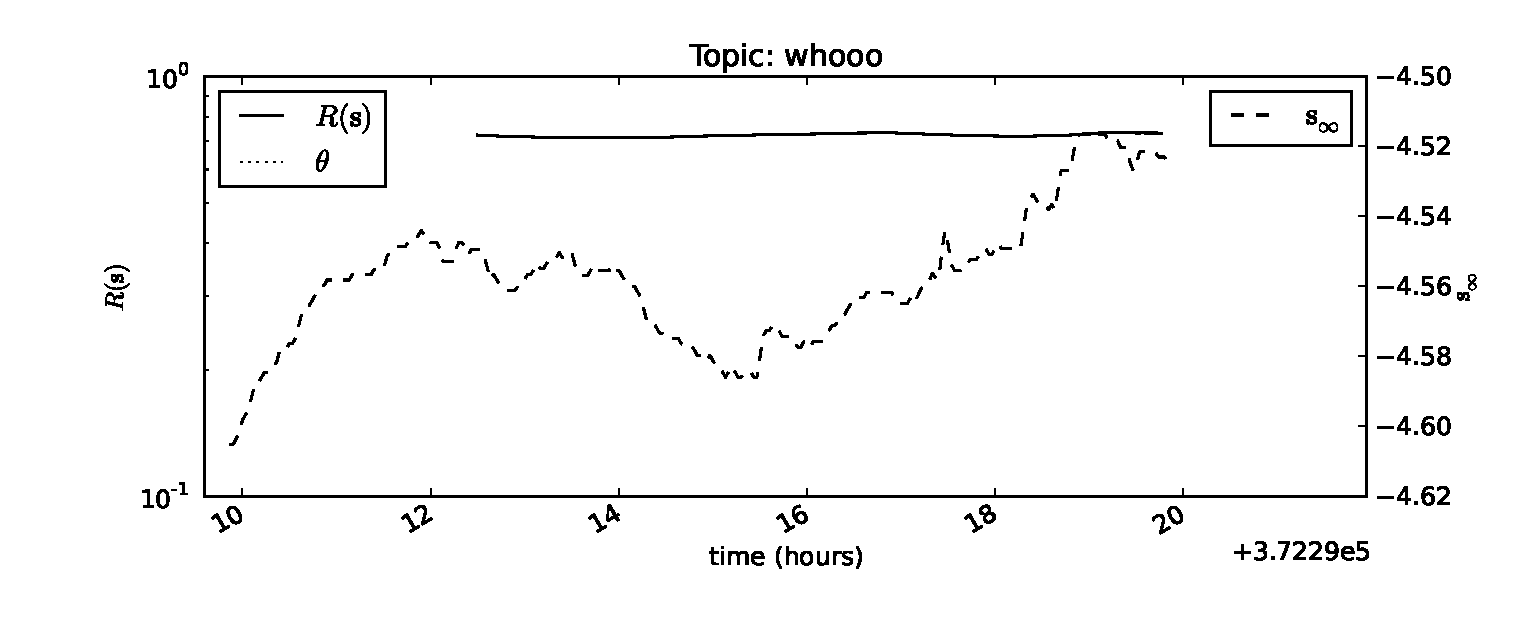
\includegraphics[height=2.5in]{../fig/final/detection_examples/tn/whooo.eps}
\end{center}
\caption{\label{fig:examples2} Examples of true negatives --- topics that did
  not trend and were not detected as trending. {\bf Top}: Although Ludacris, a
  well-known celebrity, receives constant attention on Twitter, there is no
  anomolous event involving Ludacris that would cause the topic to trend. {\bf
    Bottom}: The word ``tweetin'' is being used as a part of regular speech to
  refer to the act of posting a message on Twitter, and does not constitute a
  trending topic. }
\end{figure}

In Figure \ref{fig:examples3}, we show examples of false negatives --- topics
that were not trending, but were detected as such. It is interesting to note
that ome topics that did not trend, such as ``redsn0w'' in the bottom half of
the figure, may be associated with emerging stories of smaller magnitude that
almost became trending topics.
\begin{figure}[!h]
\begin{center}
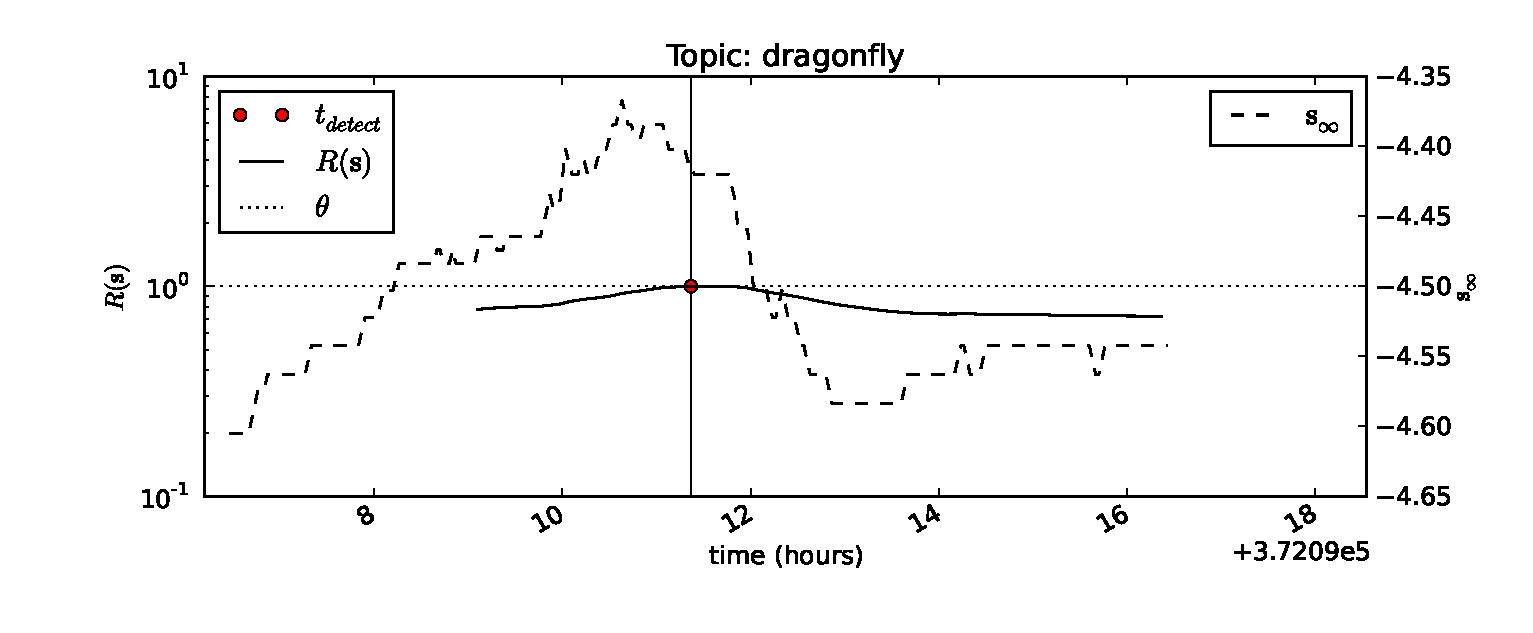
\includegraphics[height=2.5in]{../fig/final/detection_examples/fp/dragonfly.eps}
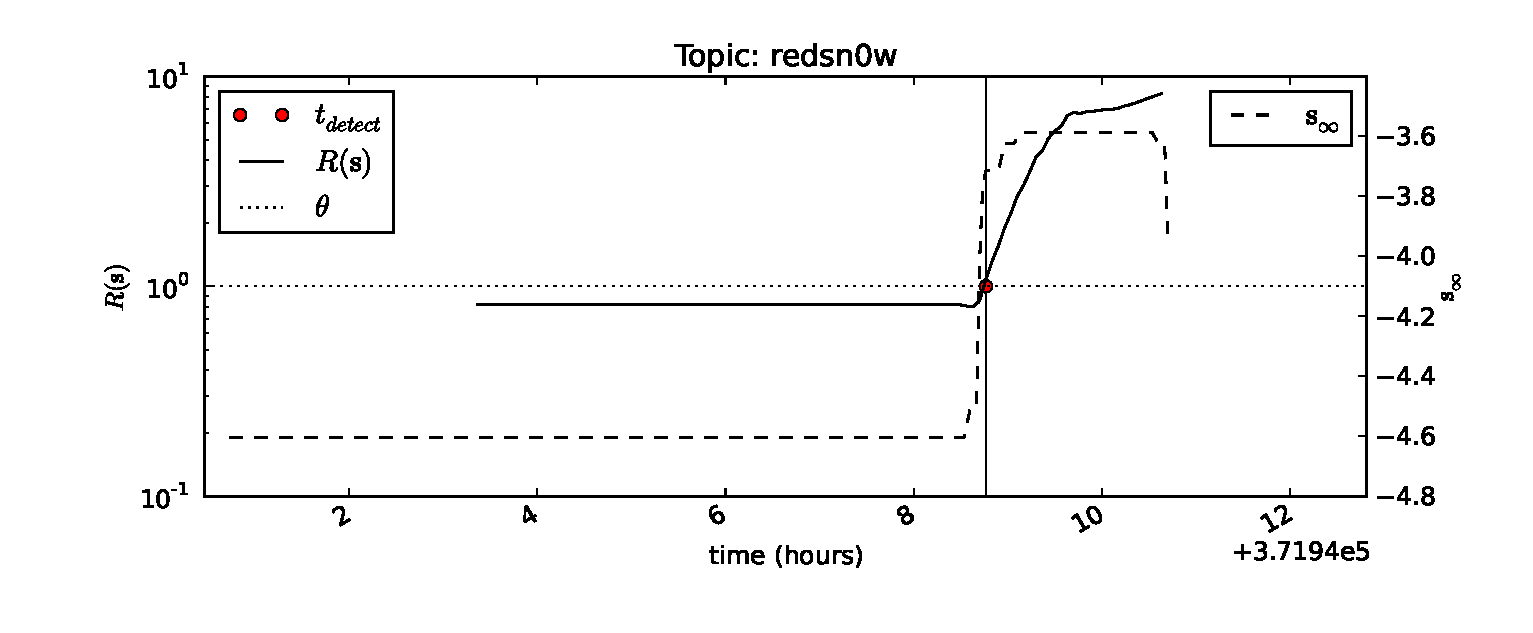
\includegraphics[height=2.5in]{../fig/final/detection_examples/fp/redsn0w.eps}
%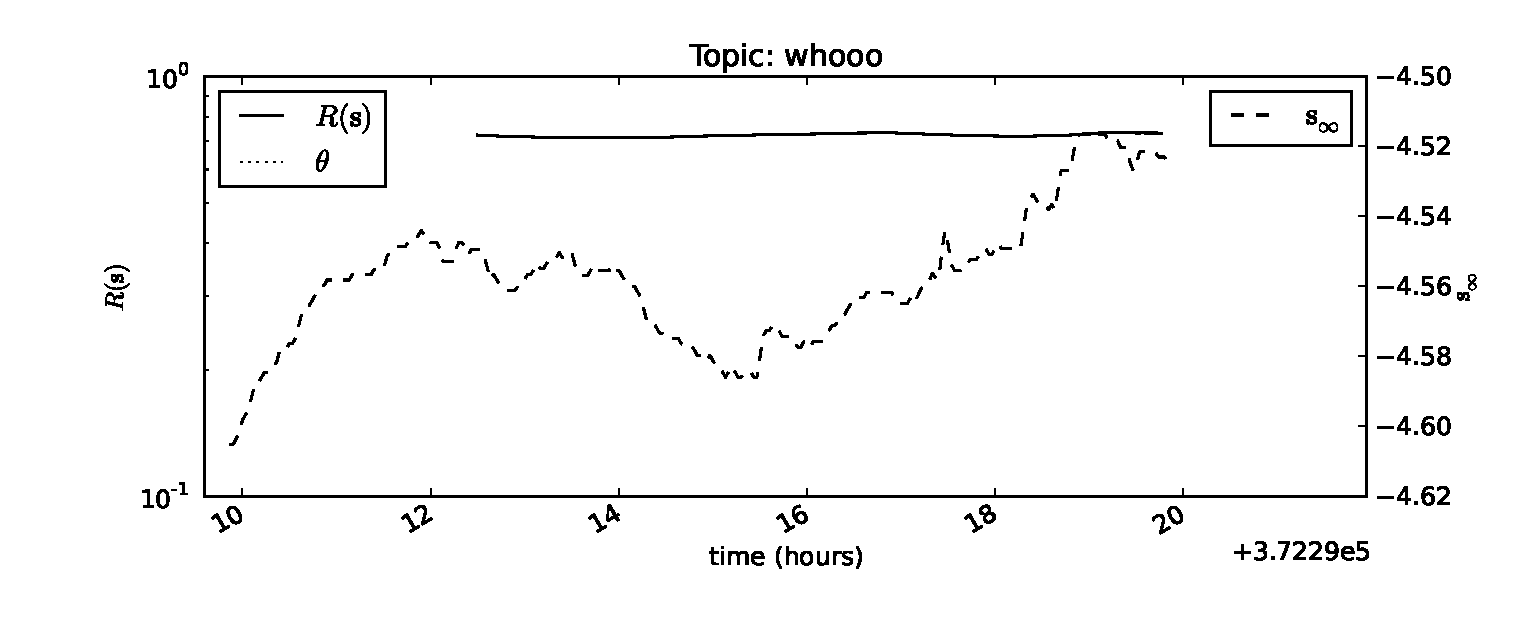
\includegraphics[height=2.5in]{../fig/final/detection_examples/tn/whooo.eps}
\end{center}
\caption{\label{fig:examples3} Examples of false positives --- topics that did
  not trend but were detected as trending. {\bf Top}: If the activity of a topic trends
  upward for a sufficiently long time, it may sufficiently resemble the activity
  of topics that trendedand lead to a false detection. {\bf Bottom}: Some false positives
  refer to actual breaking events that happened to not make the Trending Topics
  list on Twitter. The topic ``redsn0w,'' for example, coincides with a new
  release of popular jailbreaking tool for iOS.}
\end{figure}

\section{Effect of Parameters}
\subsection{Effect on Position Along ROC Curve}
\clearpage
In this section, we analyze the effect of each parameter on the position along
the ROC curve. To simplify analysis, we again consider only the top, center and
bottom regions of the curve. Table \ref{tbl:roc_pos} shows the mean of the
parameters responsible for the $(FPR,TPR)$ points in each region. It is
immediately clear that the mean threshold $\theta$ is dramatically different in
each region. This coincides with our intuition that a low threshold leads to
higher $TPR$ and $FPR$ (top region) and vice versa (bottom region). Similarly, a
higher number of required consecutive detections $D_{req}$ puts us in the bottom
region of the curve, and a lower number puts us in the center and top
regions. Another clear effect is that low values of $\gamma$ put us in the
bottom region and higher values put is in the center and top regions. $N_{obs}$, $h_{ref}$, and $N_{smooth}$ do not appear to have a
significant effect on the position along the curve.
% TODO: INTERPRET THIS. 
\begin{table}
\begin{center}
\begin{tabular}{|l|llllll|}
\hline
& $\langle N_{obs} \rangle$ & $\langle h_{ref} \rangle$ &$\langle \gamma
  \rangle$ & $\langle D_{req} \rangle$ & $\langle \theta \rangle$ & $\langle
  N_{smooth} \rangle$ \\\hline
top & 76.93 & 6.86 & 4.38 & 2.90 & 0.81 & 88.66\\
center & 77.92 & 6.09 & 3.75 & 2.88 & 1.79 & 88.61\\
bottom & 68.76 & 6.83 & 1.81 & 3.70 & 2.69 & 88.10\\
\hline
\end{tabular}
\end{center}
\caption{\label{tbl:roc_pos} The effect of parameters on position along the ROC curve.}
\end{table}

\clearpage
\subsection{Effect on Movement Along ROC Curve}
For each ROC curve, we have a parameter that varies to produce the ROC curve,
which we will call the variable paramter, and a fixed combination of the
remaining paramters, which we will call the constant parameters.

As we vary the variable parameter, how do we move up or down the ROC curve?

We show how varying a given parameter $p$ trades off $FPR$ for $TPR$ by
computing the discrete derivative of $FPR$ and $TPR$ with respect to $p$. For
each ROC curve, corresponding to the variable parameter $p$ and some fixed
combination of remaining parameters, we compute
\begin{gather}
\Delta_{p,i}^{FPR} = \frac{FPR(p_{i}) - FPR(p_{i-1})}{p_i - p_{i-1}}\\
\Delta_{p,i}^{TPR} = \frac{TPR(p_{i}) - TPR(p_{i-1})}{p_i - p_{i-1}}
\end{gather}
for each ROC curve associated with $p$ and for $i$ ranging from the second to the last value
of $p$ in increasing order. If each point on the ROC curve is produced by
multiple trials, we compute the above for all possible combinations of ROC
curves. Finally, we compute the above across all combinations of fixed
parameters.

The result is a distribution of discrete derivatives of $FPR$ and $TPR$ with
respect to a variable parameter of interest $p$ which highlights the effect of
$p$ on tradeoffs between $FPR$ and $TPR$. We can refer this effect as moving
``up'' the ROC curve, or ``down'' the ROC curve. If most of the mass of
$\Delta_{p}^{FPR}$ and $\Delta_{p}^{TPR}$ is at values greater than 0, then an
increase in $p$ causes a decrease in $FPR$ at the expense of lower $TPR$, moving
down the curve. If, on the other hand, most of the mass is at values less than
zero, an increase in $p$ causes an increase in $TPR$ at the expensive of higher
$FPR$, moving up the curve.

Sometimes, the curve moves neither toward $(0,0)$ (``down the curve'') nor
toward $(1,1)$ (``up the curve'') but toward $(0,1)$ or $(1,0)$. The former
represents an increase in $TPR$ in addition to a decrease in $FPR$ --- a win-win
situation. The latter represents the exact opposite of that --- an increase in
$FPR$ and a decrease in $TPR$.

Note that we did not count $\Delta_p$ for consecutive points at $(0,0)$ or
$(1,1)$ since the $TPR$ and $FPR$ are not free to move any further despite
changes to the variable parameter.

In Table \ref{tbl:roc_deltas}, we see the movement along the curve caused by
changes in each parameter.
\begin{table}
\begin{center}
\begin{tabular}{|l|llllll|}
\multicolumn{7}{c}{$\langle \Delta_p^{FPR} \rangle$}\\
\hline
& $N_{obs}$ & $h_{ref}$ &$\gamma$ & $D_{req}$ & $\theta$ & $N_{smooth}$\\\hline
top & -0.0023 & 0.0335 & -0.0945 & -0.0493 & -0.9807 & -0.0002\\
center & -0.0002 & 0.0413 & 0.0846 & -0.0098 & -0.0746 & 0.0001\\
bottom & 0.0002 & 0.0061 & 0.0306 & -0.0052 & N/A & 0.0001\\
\hline
\end{tabular}
\begin{tabular}{|l|llllll|}
\multicolumn{7}{c}{$\langle \Delta_p^{TPR} \rangle$}\\
\hline
& $N_{obs}$ & $h_{ref}$ &$\gamma$ & $D_{req}$ & $\theta$ & $N_{smooth}$\\\hline
top & -0.0002 & 0.0019 & -0.0126 & -0.0228 & -0.2298 & -0.0001\\
center & 0.0003 & -0.0007 & 0.0227 & -0.0358 & -0.0238 & 0.0000\\
bottom & 0.0016 & -0.0168 & 0.3838 & -0.0594 & N/A & 0.0004\\
\hline
\end{tabular}
\end{center}
\caption{\label{tbl:roc_deltas} Movement along ROC curve caused by changes in
  each parameter, depending on which region in the $FPR$-$TPR$ plane the ROC
  curve starts.}
%TODO: Transpose this if you have time to make it parameter-centric rather than
%position centric.
\end{table}
The behavior is not uniform, however. The change in
$FPR$ and $TPR$ depending on the current position in the $FPR$-$TPR$ plane. To
study the effect of initial position on the movement along the curve, we once
again break the space up into top, center and bottom regions. This time, each
ROC curve is assigned to a region based on where the ROC curve begins (starting
with the lowest value of the variable parameter). The discrete derivatives
resulting from that curve are then assigned to the appropriate region.

It is not surprising that $\theta$, which has the most influence on the position
along the curve, also has by far the most influence on the movement along the
curve. A larger $\theta$ moves us down the curve no matter where we start, as
expected. Similarly, a larger $D_{req}$ always moves us down the curve, also as
expected. 

Also influential is $\gamma$. Interestingly, it moves us down the curve
if we start in the top region, and up the curve otherwise. 

%TODO: Interpret!

An increase in $N_{obs}$ causes us to move down the curve if we start in the top
region and up the curve if we start in the bottom region. In the center, region,
it causes a slight movement perpendicular to the curve --- increasing $TPR$
while decreasing $FPR$.

The length of the reference signals in hours and half the time window for a
single detection run, $h_{ref}$ causes us to move down the curve if we start in
the bottom and up the curve if we start in the top.

$N_{smooth}$ has no significant effect for the range of smoothing widths
explored. It is possible that a bigger difference may be seen outside of this
range.

\section{Recommendations}

We propose parameter regimes appropriate for the following three situations: 1)
the cost of a false positive outweighs the cost of a false negative, 2) the cost
of a false negative outweighs the cost of a false positive, and 3) the costs of
a false positive and a false negative are comparable. We make use of the results
involving position and movement along a the ROC curve shown in the previous
sections.

\subsection{Cost($FP$) $\ll$ Cost($TP$)}
We recommend the parameter settings in the third row of Table \ref{tbl:roc_pos},
corresponding to the bottom region, which give an average $(FPR,TPR)$ equal to
$(0.02,0.27)$. For fine-tuning, we can increase $h_{ref}$ or decrease $\gamma$ or
$N_{obs}$ to move down the curve (or do the opposite to move up the curve.)

\subsection{Cost($FP$) $\gg$ Cost($TP$)}
We recommend the parameter settings in the first row of Table \ref{tbl:roc_pos},
corresponding to the top region, which give an average $(FPR,TPR)$ equal to
$(0.74,0.98)$. For fine-tuning, we can decrease $h_{ref}$ or increase $\gamma$,
$N_{obs}$ to move up the curve (or do the opposite to move down the curve.)

\subsection{Cost($FP$) $\sim$ Cost($TP$)}
We recommend the parameter settings in the second row of Table
\ref{tbl:roc_pos}, corresponding to the center region, which give an average
$(FPR,TPR)$ equal to $(0.10,0.87)$. For fine-tuning, we can increase $N_{obs}$
to simultaneously increase $TPR$ and decrease $FPR$.

